\clearpage
\subsection{実習3-2 可変抵抗(ポテンショメータ)の電圧電流特性}
\begin{itemize}
	\item プログラム\ref{ex32-block}は可変抵抗端子1-2間の電圧電流特性を計測するプログラムである.
	\item 全ての場合において,$R_{0}$の値は10\,k\rm{$\Omega$}とした.
	\item 実行後,フロントパネルは\wfig{ex32-flont}のようになり,計測結果は\wtab{ER1-2}のようになった.
	\item 計測データを基に作成した電圧電流特性のグラフは\wfig{3-2-1}である.
	\item 端子2-3間では,\wtab{ER2-3},\wfig{3-2-2}.端子3-1間では,\wtab{ER3-1},\wfig{3-2-3}となった.
\end{itemize}

\begin{figure}[h]
\centering
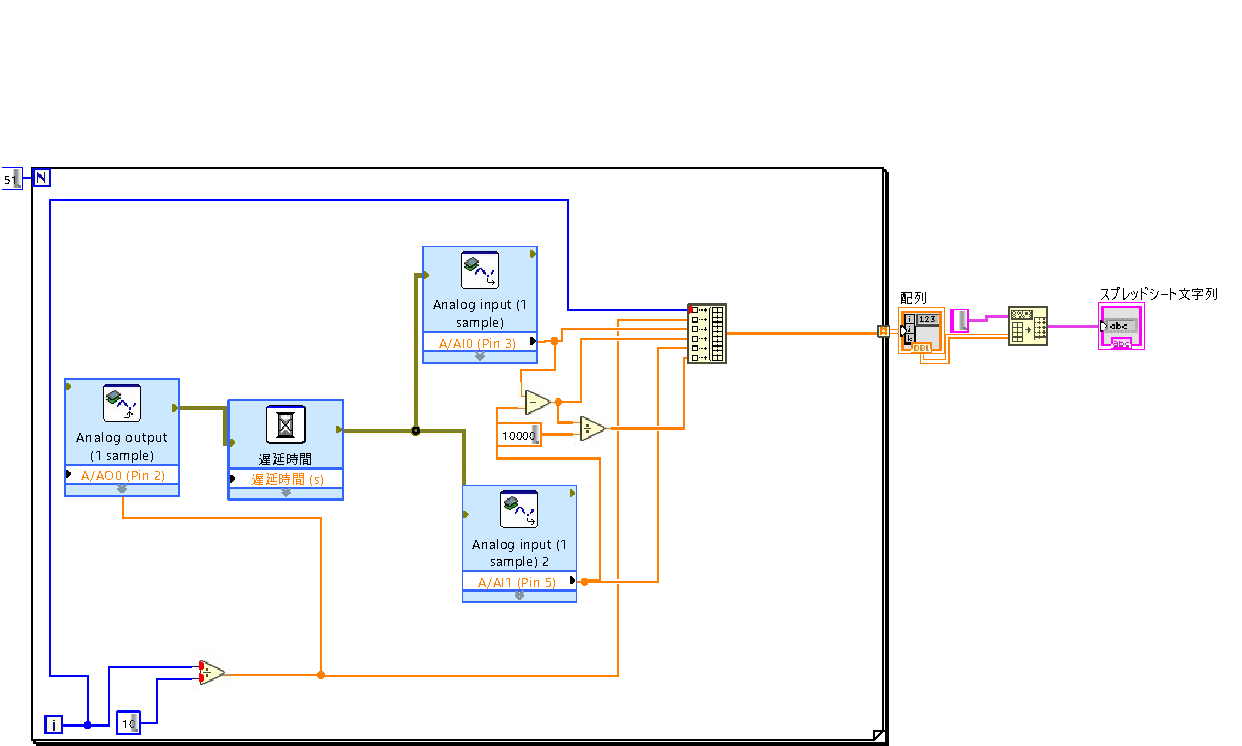
\includegraphics[scale=0.5]{./fig/ex32-block.pdf}\\
\useMycounter[\label{ex32-block}]可変抵抗の電圧電流特性計測時のブロックダイアグラム
\end{figure}

\begin{figure}[h]
\centering
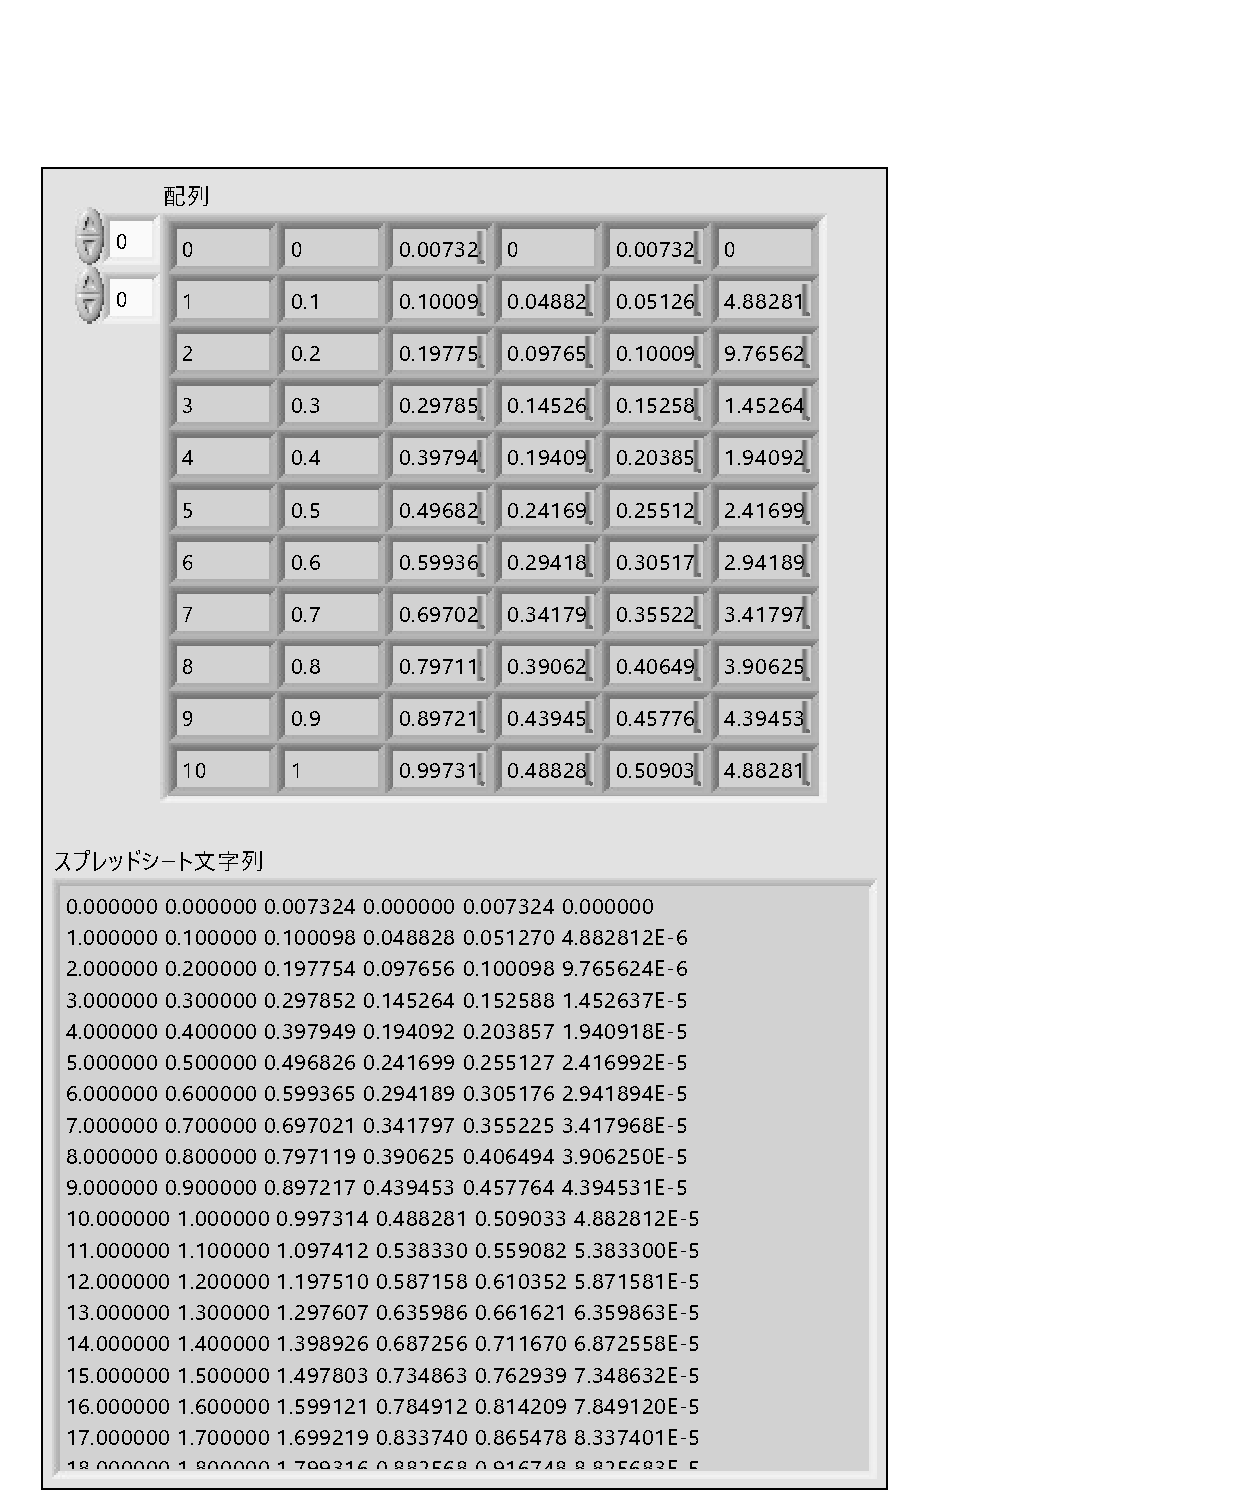
\includegraphics[scale=0.5]{./fig/ex32-flont.pdf}
\caption{可変抵抗の電圧電流特性測定時のフロントパネル}
\label{fig:ex32-flont}
\end{figure}

\begin{table}[h]
\centering
\caption{可変抵抗器(1-2端子間)の諸特性値}
\label{tab:ER1-2}
\scalebox{0.8}{
\begin{tabular}{ccccccc}
\hline
カウンタ変数 & Aでの$V_{U}$[\rm{V}] & Aでの$I_{U}$[\rm{A}] & Bでの$V_{U}$[\rm{V}]    & Bでの$I_{U}$[\rm{A}]   & Cでの$V_{U}$[\rm{V}]& Cでの$I_{U}$[\rm{A}] \\
\hline
  0      & 0.007324 & 0.00000012 & 0.006104 & 0.00000024 & 0.006104 & 0.00000024 \\
  1      & 0.048828 & 0.00000513 & 0.031738 & 0.00000696 & 0.007324 & 0.00000903 \\
  2      & 0.098877 & 0.00000977 & 0.065918 & 0.00001306 & 0.006104 & 0.00001892 \\
  3      & 0.151367 & 0.00001453 & 0.100098 & 0.00001953 & 0.006104 & 0.00002930 \\
  4      & 0.203857 & 0.00001929 & 0.133057 & 0.00002637 & 0.006104 & 0.00003894 \\
  5      & 0.253906 & 0.00002441 & 0.168457 & 0.00003296 & 0.006104 & 0.00004932 \\
  6      & 0.305176 & 0.00002930 & 0.201416 & 0.00003979 & 0.007324 & 0.00005920 \\
  7      & 0.355225 & 0.00003418 & 0.234375 & 0.00004639 & 0.007324 & 0.00006897 \\
  8      & 0.406494 & 0.00003918 & 0.268555 & 0.00005286 & 0.007324 & 0.00007910 \\
  9      & 0.456543 & 0.00004407 & 0.301514 & 0.00005957 & 0.007324 & 0.00008911 \\
  10     & 0.507812 & 0.00004907 & 0.336914 & 0.00006616 & 0.007324 & 0.00009888 \\
  11     & 0.559082 & 0.00005396 & 0.369873 & 0.00007275 & 0.006104 & 0.00010900 \\
  12     & 0.610352 & 0.00005859 & 0.404053 & 0.00007947 & 0.006104 & 0.00011900 \\
  13     & 0.661621 & 0.00006360 & 0.438232 & 0.00008606 & 0.006104 & 0.00012900 \\
  14     & 0.712891 & 0.00006848 & 0.472412 & 0.00009253 & 0.006104 & 0.00013900 \\
  15     & 0.762939 & 0.00007349 & 0.505371 & 0.00009924 & 0.006104 & 0.00014900 \\
  16     & 0.814209 & 0.00007849 & 0.539551 & 0.00010600 & 0.006104 & 0.00015900 \\
  17     & 0.865478 & 0.00008350 & 0.57251  & 0.00011300 & 0.007324 & 0.00016900 \\
  18     & 0.915527 & 0.00008838 & 0.606689 & 0.00011900 & 0.007324 & 0.00017900 \\
  19     & 0.966797 & 0.00009302 & 0.640869 & 0.00012600 & 0.007324 & 0.00018900 \\
  20     & 1.018066 & 0.00009790 & 0.673828 & 0.00013200 & 0.007324 & 0.00019900 \\
  21     & 1.068115 & 0.00010300 & 0.709228 & 0.00013900 & 0.007324 & 0.00020900 \\
  22     & 1.119385 & 0.00010800 & 0.742187 & 0.00014600 & 0.008545 & 0.00021900 \\
  23     & 1.170654 & 0.00011300 & 0.775146 & 0.00015200 & 0.008545 & 0.00022900 \\
  24     & 1.221924 & 0.00011800 & 0.809326 & 0.00015900 & 0.008545 & 0.00023900 \\
  25     & 1.273193 & 0.00012200 & 0.843506 & 0.00016600 & 0.008545 & 0.00024900 \\
  26     & 1.324463 & 0.00012700 & 0.877685 & 0.00017200 & 0.008545 & 0.00025900 \\
  27     & 1.374512 & 0.00013200 & 0.910644 & 0.00017900 & 0.009766 & 0.00026900 \\
  28     & 1.425781 & 0.00013700 & 0.944824 & 0.00018600 & 0.009766 & 0.00027900 \\
  29     & 1.477051 & 0.00014200 & 0.979004 & 0.00019200 & 0.008545 & 0.00028900 \\
  30     & 1.527099 & 0.00014700 & 1.013183 & 0.00019900 & 0.009766 & 0.00029900 \\
  31     & 1.57959  & 0.00015200 & 1.046142 & 0.00020500 & 0.010986 & 0.00030900 \\
  32     & 1.630859 & 0.00015700 & 1.080322 & 0.00021200 & 0.012207 & 0.00031900 \\
  33     & 1.680908 & 0.00016200 & 1.114502 & 0.00021900 & 0.010986 & 0.00032900 \\
  34     & 1.730957 & 0.00016700 & 1.147461 & 0.00022500 & 0.013428 & 0.00033900 \\
  35     & 1.782226 & 0.00017200 & 1.181641 & 0.00023200 & 0.012207 & 0.00034900 \\
  36     & 1.834717 & 0.00017600 & 1.21582  & 0.00023800 & 0.013428 & 0.00035900 \\
  37     & 1.885986 & 0.00018100 & 1.25     & 0.00024500 & 0.013428 & 0.00036900 \\
  38     & 1.936035 & 0.00018600 & 1.28418  & 0.00025200 & 0.014648 & 0.00037900 \\
  39     & 1.987304 & 0.00019100 & 1.317139 & 0.00025800 & 0.014648 & 0.00038900 \\
  40     & 2.038574 & 0.00019600 & 1.351318 & 0.00026500 & 0.014648 & 0.00039800 \\
  41     & 2.089844 & 0.00020100 & 1.385498 & 0.00027200 & 0.015869 & 0.00040800 \\
  42     & 2.141113 & 0.00020600 & 1.419678 & 0.00027800 & 0.015869 & 0.00041800 \\
  43     & 2.192383 & 0.00021100 & 1.453857 & 0.00028500 & 0.015869 & 0.00042800 \\
  44     & 2.241211 & 0.00021600 & 1.486816 & 0.00029100 & 0.015869 & 0.00043800 \\
  45     & 2.29248  & 0.00022100 & 1.520996 & 0.00029800 & 0.015869 & 0.00044800 \\
  46     & 2.34497  & 0.00022500 & 1.555176 & 0.00030400 & 0.01709  & 0.00045800 \\
  47     & 2.39624  & 0.00023000 & 1.589355 & 0.00031100 & 0.01709  & 0.00046800 \\
  48     & 2.446289 & 0.00023500 & 1.623535 & 0.00031800 & 0.01709  & 0.00047800 \\
49     & 2.495117 & 0.00024100 & 1.657715 & 0.00032400 & 0.01709  & 0.00048800 \\
50     & 2.547607 & 0.00024500 & 1.689453 & 0.00033100 & 0.018311 & 0.00049800 \\
\hline
\end{tabular}
}
\end{table}

\begin{table}[h]
\centering
\caption{可変抵抗器(2-3端子間)の諸特性値}
\label{tab:ER2-3}
     \scalebox{0.8}{
    \begin{tabular}{ccccccc}
    \hline
	カウンタ変数 & Aでの$V_{U}$[\rm{V}] & Aでの$I_{U}$[\rm{A}] & Bでの$V_{U}$[\rm{V}]   & Bでの$I_{U}$[\rm{A}]   & Cでの$V_{U}$[\rm{V}] & Cでの$I_{U}$[\rm{A}]\\
	\hline
	0      & 0.006104 & 0.00000024 & 0.006104 & 0.00000012 & 0.007324 & 0.00000000 \\
	1      & 0.007324 & 0.00000891 & 0.0354   & 0.00000610 & 0.050049 & 0.00000488 \\
	2      & 0.007324 & 0.00001892 & 0.070801 & 0.00001257 & 0.101318 & 0.00000964 \\
	3      & 0.009766 & 0.00002881 & 0.108643 & 0.00001868 & 0.151367 & 0.00001453 \\
	4      & 0.012207 & 0.00003870 & 0.144043 & 0.00002539 & 0.202637 & 0.00001953 \\
	5      & 0.015869 & 0.00004822 & 0.180664 & 0.00003174 & 0.253906 & 0.00002441 \\
	6      & 0.019531 & 0.00005774 & 0.217285 & 0.00003796 & 0.305176 & 0.00002930 \\
	7      & 0.023193 & 0.00006738 & 0.252686 & 0.00004468 & 0.356445 & 0.00003406 \\
	8      & 0.028076 & 0.00007690 & 0.289307 & 0.00005078 & 0.407715 & 0.00003894 \\
	9      & 0.031738 & 0.00008655 & 0.325928 & 0.00005713 & 0.457764 & 0.00004395 \\
	10     & 0.0354   & 0.00009619 & 0.363769 & 0.00006335 & 0.509033 & 0.00004895 \\
	11     & 0.039062 & 0.00010600 & 0.39917  & 0.00006982 & 0.560303 & 0.00005371 \\
	12     & 0.042725 & 0.00011600 & 0.435791 & 0.00007617 & 0.610352 & 0.00005872 \\
	13     & 0.046387 & 0.00012500 & 0.472412 & 0.00008264 & 0.661621 & 0.00006360 \\
	14     & 0.05127  & 0.00013500 & 0.507812 & 0.00008911 & 0.712891 & 0.00006860 \\
	15     & 0.054932 & 0.00014400 & 0.544434 & 0.00009521 & 0.762939 & 0.00007349 \\
	16     & 0.058594 & 0.00015400 & 0.581055 & 0.00010200 & 0.81543  & 0.00007825 \\
	17     & 0.063477 & 0.00016300 & 0.618896 & 0.00010800 & 0.865478 & 0.00008325 \\
	18     & 0.067139 & 0.00017300 & 0.655518 & 0.00011400 & 0.916748 & 0.00008826 \\
	19     & 0.072021 & 0.00018200 & 0.690918 & 0.00012100 & 0.966797 & 0.00009326 \\
	20     & 0.075684 & 0.00019200 & 0.727539 & 0.00012700 & 1.018066 & 0.00009814 \\
	21     & 0.080566 & 0.00020200 & 0.762939 & 0.00013300 & 1.068115 & 0.00010300 \\
	22     & 0.084229 & 0.00021100 & 0.79956  & 0.00014000 & 1.120605 & 0.00010800 \\
	23     & 0.089111 & 0.00022100 & 0.836182 & 0.00014600 & 1.170654 & 0.00011300 \\
	24     & 0.093994 & 0.00023000 & 0.872803 & 0.00015300 & 1.221924 & 0.00011800 \\
	25     & 0.097656 & 0.00024000 & 0.909424 & 0.00015900 & 1.273193 & 0.00012300 \\
	26     & 0.102539 & 0.00025000 & 0.946045 & 0.00016500 & 1.324463 & 0.00012700 \\
	27     & 0.107422 & 0.00025900 & 0.982666 & 0.00017200 & 1.375732 & 0.00013200 \\
	28     & 0.111084 & 0.00026900 & 1.018066 & 0.00017800 & 1.425781 & 0.00013700 \\
	29     & 0.114746 & 0.00027800 & 1.054687 & 0.00018400 & 1.478271 & 0.00014200 \\
	30     & 0.119629 & 0.00028800 & 1.091308 & 0.00019100 & 1.52832  & 0.00014700 \\
  	31     & 0.123291 & 0.00029800 & 1.12793  & 0.00019700 & 1.57959  & 0.00015200 \\
	32     & 0.128174 & 0.00030700 & 1.164551 & 0.00020300 & 1.629639 & 0.00015700 \\
 	33     & 0.135498 & 0.00031600 & 1.199951 & 0.00021000 & 1.680908 & 0.00016200 \\
 	34     & 0.140381 & 0.00032600 & 1.237793 & 0.00021600 & 1.733398 & 0.00016700 \\
 	35     & 0.144043 & 0.00033600 & 1.274414 & 0.00022300 & 1.784668 & 0.00017200 \\
 	36     & 0.150146 & 0.00034500 & 1.311035 & 0.00022900 & 1.834717 & 0.00017700 \\
 	37     & 0.155029 & 0.00035400 & 1.347656 & 0.00023500 & 1.887207 & 0.00018100 \\
	38     & 0.159912 & 0.00036400 & 1.383056 & 0.00024200 & 1.937256 & 0.00018600 \\
 	39     & 0.166016 & 0.00037300 & 1.420898 & 0.00024800 & 1.987304 & 0.00019100 \\
	40     & 0.170898 & 0.00038300 & 1.456299 & 0.00025400 & 2.039795 & 0.00019600 \\
	41     & 0.175781 & 0.00039200 & 1.49292  & 0.00026100 & 2.091064 & 0.00020100 \\
	42     & 0.180664 & 0.00040200 & 1.530762 & 0.00026700 & 2.141113 & 0.00020600 \\
	43     & 0.184326 & 0.00041200 & 1.566162 & 0.00027300 & 2.192383 & 0.00021100 \\
	44     & 0.189209 & 0.00042100 & 1.602783 & 0.00028000 & 2.243652 & 0.00021500 \\
	45     & 0.194092 & 0.00043000 & 1.638183 & 0.00028600 & 2.294922 & 0.00022000 \\
	46     & 0.197754 & 0.00044000 & 1.676025 & 0.00029200 & 2.346191 & 0.00022500 \\
	47     & 0.201416 & 0.00045000 & 1.711426 & 0.00029900 & 2.39624  & 0.00023000 \\
	48     & 0.20752  & 0.00045900 & 1.749267 & 0.00030500 & 2.44751  & 0.00023500 \\
	49     & 0.213623 & 0.00046800 & 1.784668 & 0.00031200 & 2.497558 & 0.00024000 \\
	50     & 0.218506 & 0.00047800 & 1.821289 & 0.00031800 & 2.548828 & 0.00024500 \\
\hline
  \end{tabular}
  }
  \end{table}

\begin{table}[h]
  \centering
    \caption{可変抵抗器(3-1端子間)の諸特性値}
    \label{tab:ER3-1}
     \scalebox{0.8}{
    \begin{tabular}{ccccccc}
    \hline
カウンタ変数 & Aでの$V_{U}$[\rm{V}] & Aでの$I_{U}$[\rm{A}] & Bでの$V_{U}$[\rm{V}] & Bでの$I_{U}$[\rm{A}]   & Cでの$V_{U}$[\rm{V}] & Cでの$I_{U}$[\rm{A}]\\
\hline
  0         & 0.007324       & 0.00000000 & 0.00732400 & 0.00000012 & 0.00732400 & 0.00000012 \\
  1         & 0.050049       & 0.00000488 & 0.04882800 & 0.00000513 & 0.05127000 & 0.00000500 \\
  2         & 0.101318       & 0.00000964 & 0.10009800 & 0.00000964 & 0.10376000 & 0.00000940 \\
  3         & 0.151367       & 0.00001465 & 0.15136700 & 0.00001465 & 0.15258800 & 0.00001453 \\
  4         & 0.202637       & 0.00001953 & 0.20263700 & 0.00001965 & 0.20629900 & 0.00001892 \\
  5         & 0.252686       & 0.00002454 & 0.25390600 & 0.00002441 & 0.25634800 & 0.00002429 \\
  6         & 0.305176       & 0.00002917 & 0.30395500 & 0.00002942 & 0.31005900 & 0.00002856 \\
  7         & 0.355225       & 0.00003394 & 0.35522500 & 0.00003418 & 0.36010700 & 0.00003381 \\
  8         & 0.406494       & 0.00003882 & 0.40649400 & 0.00003906 & 0.41259800 & 0.00003845 \\
  9         & 0.456543       & 0.00004407 & 0.45654300 & 0.00004395 & 0.46264600 & 0.00004358 \\
  10        & 0.507812       & 0.00004895 & 0.50781200 & 0.00004919 & 0.51757800 & 0.00004810 \\
  11        & 0.559082       & 0.00005396 & 0.55786100 & 0.00005420 & 0.56762700 & 0.00005310 \\
  12        & 0.610352       & 0.00005859 & 0.60913100 & 0.00005884 & 0.62011700 & 0.00005774 \\
  13        & 0.661621       & 0.00006348 & 0.66162100 & 0.00006360 & 0.67138700 & 0.00006274 \\
  14        & 0.71167        & 0.00006885 & 0.71167000 & 0.00006860 & 0.72387700 & 0.00006738 \\
  15        & 0.762939       & 0.00007336 & 0.76293900 & 0.00007349 & 0.77514600 & 0.00007227 \\
  16        & 0.81543        & 0.00007825 & 0.81298800 & 0.00007849 & 0.82763700 & 0.00007727 \\
  17        & 0.865478       & 0.00008325 & 0.86425800 & 0.00008350 & 0.87890600 & 0.00008191 \\
  18        & 0.916748       & 0.00008826 & 0.91552700 & 0.00008826 & 0.93017600 & 0.00008691 \\
  19        & 0.966797       & 0.00009326 & 0.96557600 & 0.00009302 & 0.98266600 & 0.00009155 \\
  20        & 1.016846       & 0.00009814 & 1.01684600 & 0.00009814 & 1.03393500 & 0.00009631 \\
  21        & 1.069336       & 0.00010300 & 1.06811500 & 0.00010300 & 1.08520500 & 0.00010100 \\
  22        & 1.120605       & 0.00010800 & 1.11938500 & 0.00010800 & 1.13647400 & 0.00010600 \\
  23        & 1.170654       & 0.00011300 & 1.17065400 & 0.00011300 & 1.18896500 & 0.00011100 \\
  24        & 1.221924       & 0.00011800 & 1.22070300 & 0.00011800 & 1.24023400 & 0.00011600 \\
  25        & 1.273193       & 0.00012300 & 1.27319300 & 0.00012300 & 1.29272400 & 0.00012000 \\
  26        & 1.324463       & 0.00012700 & 1.32324200 & 0.00012800 & 1.34399400 & 0.00012600 \\
  27        & 1.375732       & 0.00013200 & 1.37329100 & 0.00013200 & 1.39648400 & 0.00013000 \\
  28        & 1.427002       & 0.00013700 & 1.42334000 & 0.00013800 & 1.44897400 & 0.00013500 \\
  29        & 1.478271       & 0.00014200 & 1.47583000 & 0.00014200 & 1.49902300 & 0.00014000 \\
  30        & 1.52832        & 0.00014700 & 1.52587900 & 0.00014700 & 1.55273400 & 0.00014500 \\
  31        & 1.57959        & 0.00015200 & 1.57836900 & 0.00015200 & 1.60400400 & 0.00015000 \\
  32        & 1.629639       & 0.00015700 & 1.62841800 & 0.00015700 & 1.65649400 & 0.00015400 \\
  33        & 1.682129       & 0.00016200 & 1.67968700 & 0.00016200 & 1.70654300 & 0.00015900 \\
  34        & 1.733398       & 0.00016700 & 1.73095700 & 0.00016700 & 1.75903300 & 0.00016400 \\
  35        & 1.783447       & 0.00017200 & 1.78100600 & 0.00017200 & 1.81152300 & 0.00016900 \\
  36        & 1.834717       & 0.00017700 & 1.83349600 & 0.00017700 & 1.86279300 & 0.00017400 \\
  37        & 1.887207       & 0.00018100 & 1.88354500 & 0.00018200 & 1.91528300 & 0.00017800 \\
  38        & 1.937256       & 0.00018600 & 1.93481400 & 0.00018700 & 1.96533200 & 0.00018400 \\
  39        & 1.987304       & 0.00019100 & 1.98486300 & 0.00019200 & 2.01782200 & 0.00018800 \\
  40        & 2.039795       & 0.00019600 & 2.03613300 & 0.00019700 & 2.07153300 & 0.00019300 \\
  41        & 2.089844       & 0.00020100 & 2.08618100 & 0.00020200 & 2.12280300 & 0.00019800 \\
  42        & 2.141113       & 0.00020600 & 2.13745100 & 0.00020600 & 2.17407200 & 0.00020300 \\
  43        & 2.192383       & 0.00021100 & 2.18994100 & 0.00021100 & 2.22656200 & 0.00020700 \\
  44        & 2.243652       & 0.00021500 & 2.23999000 & 0.00021600 & 2.27661100 & 0.00021200 \\
  45        & 2.293701       & 0.00022100 & 2.29126000 & 0.00022100 & 2.32910100 & 0.00021700 \\
  46        & 2.34497        & 0.00022500 & 2.34130800 & 0.00022600 & 2.38037100 & 0.00022200 \\
  47        & 2.39624        & 0.00023000 & 2.39379900 & 0.00023100 & 2.43164000 & 0.00022700 \\
  48        & 2.44751        & 0.00023500 & 2.44384700 & 0.00023600 & 2.48535100 & 0.00023100 \\
  49        & 2.497558       & 0.00024000 & 2.49511700 & 0.00024000 & 2.53662100 & 0.00023600 \\
  50        & 2.547607       & 0.00024500 & 2.54638600 & 0.00024500 & 2.58789000 & 0.00024100 \\
\hline
\end{tabular}
    }
\end{table}

\begin{figure}[h]
  %\begin{minipage}[c]{0.5\hsize}
    \centering
    \subfloat{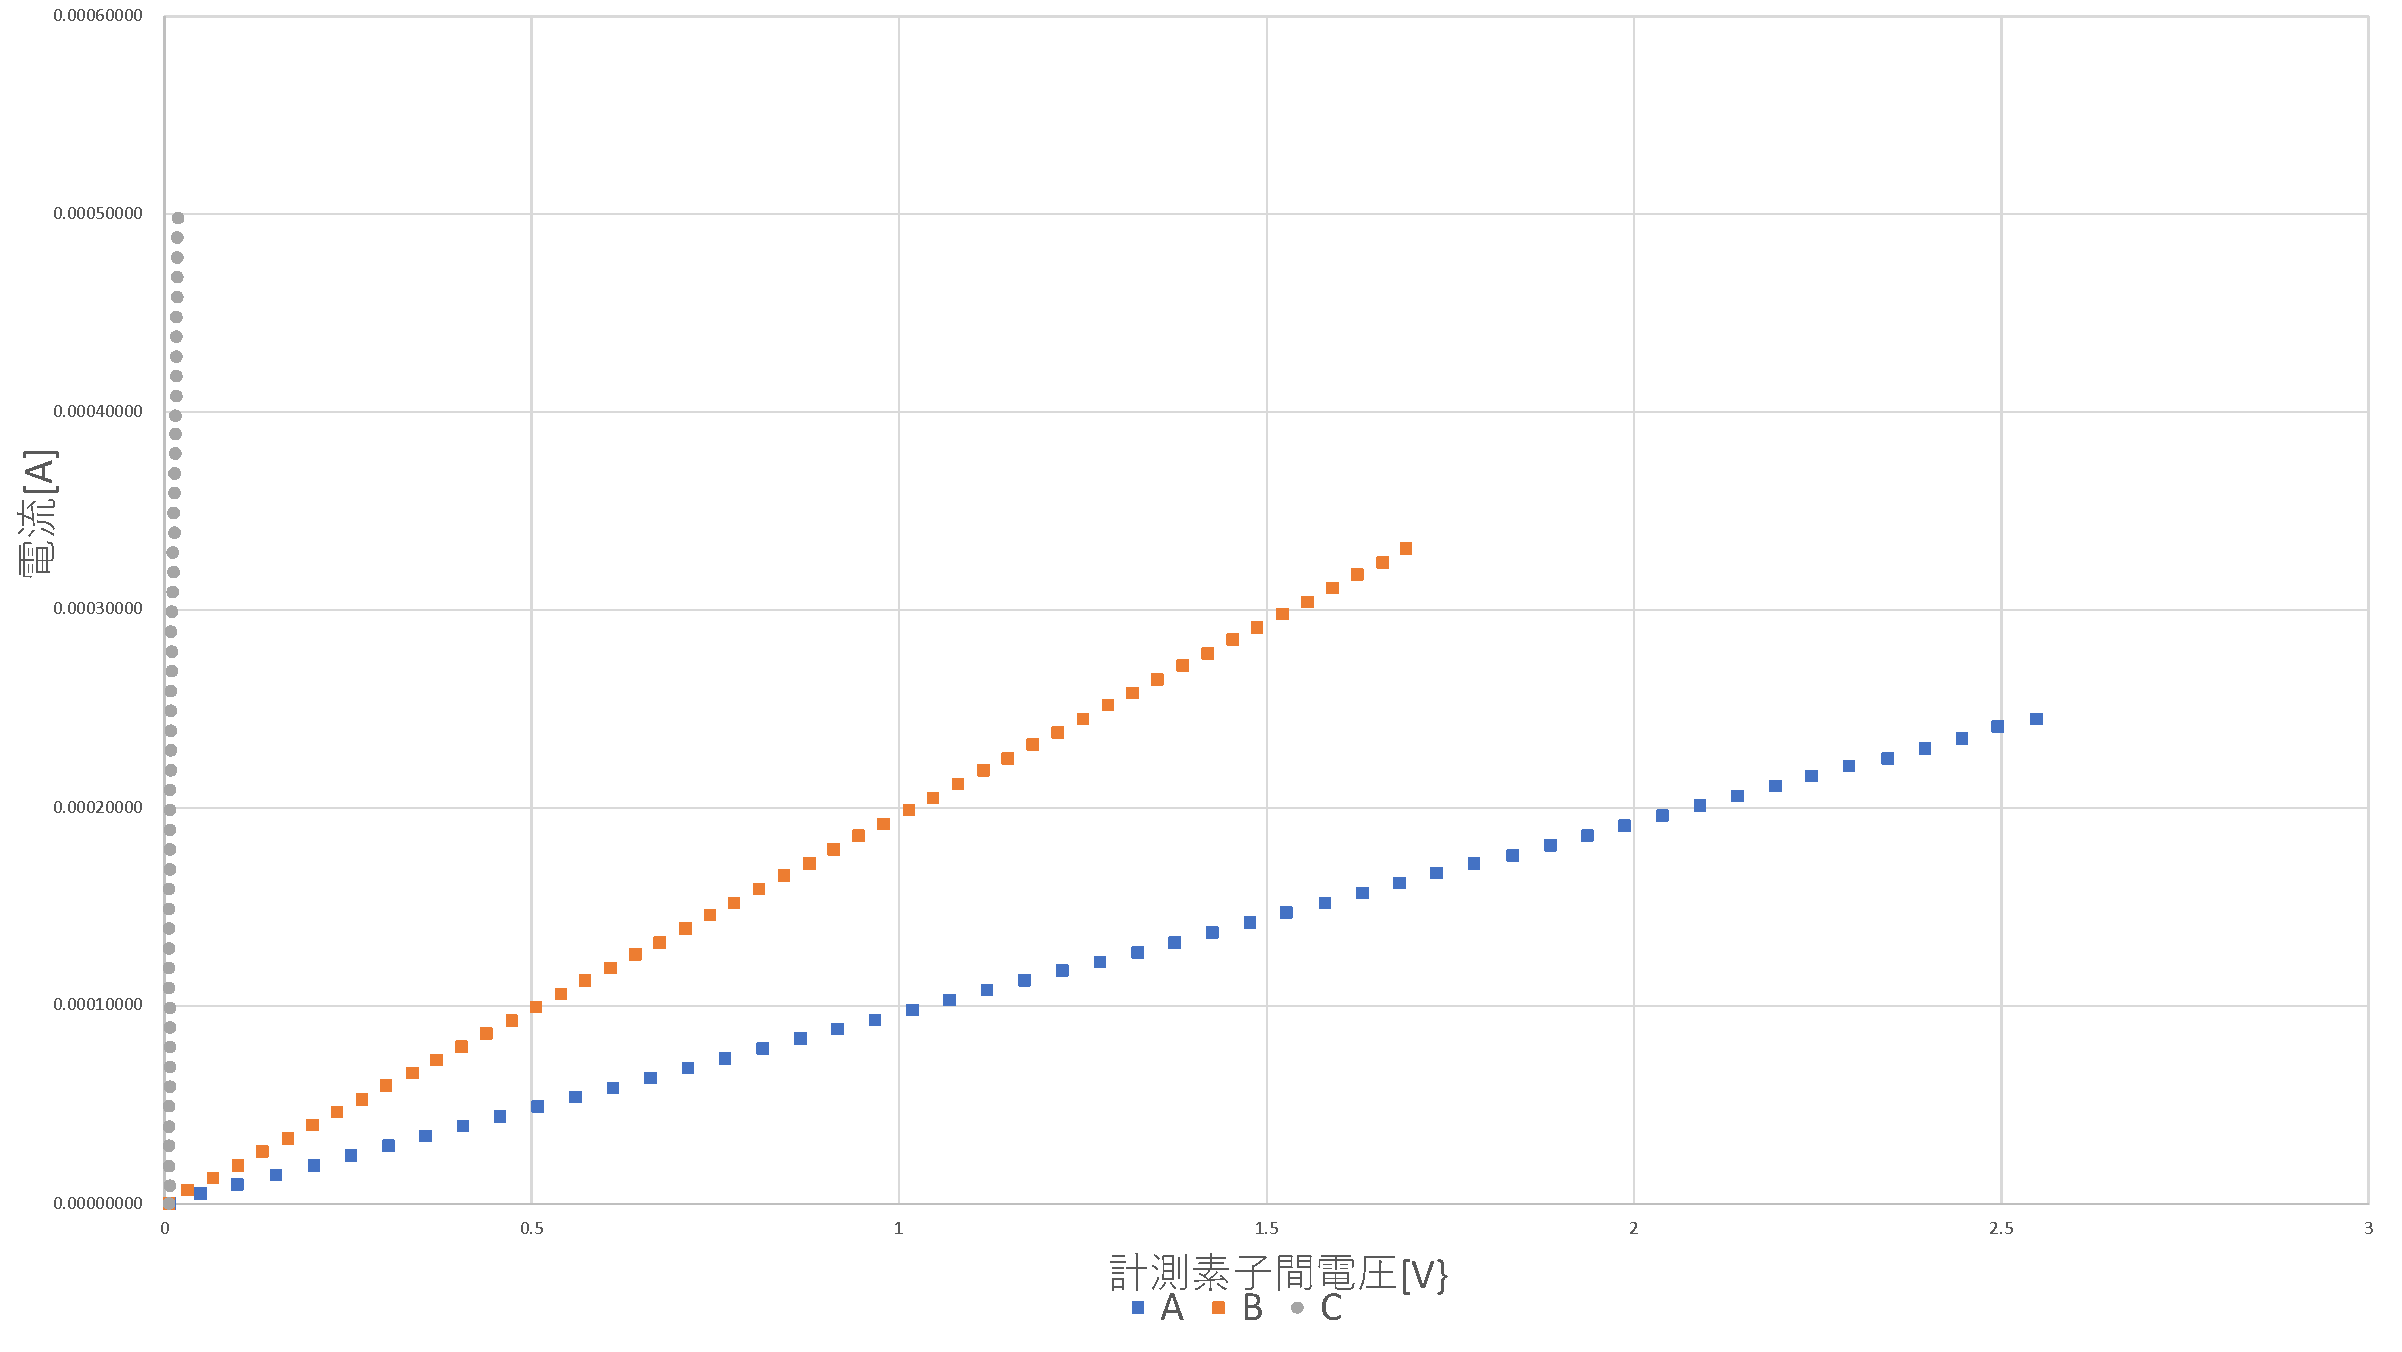
\includegraphics[scale=0.315]{./fig/3-2-1.pdf}}
	\caption{可変抵抗器(1-2端子間)の電圧電流特性}
	\label{fig:3-2-1}
	%\end{minipage}
  %\begin{minipage}[c]{0.5\hsize}
    \centering
   \subfloat{ 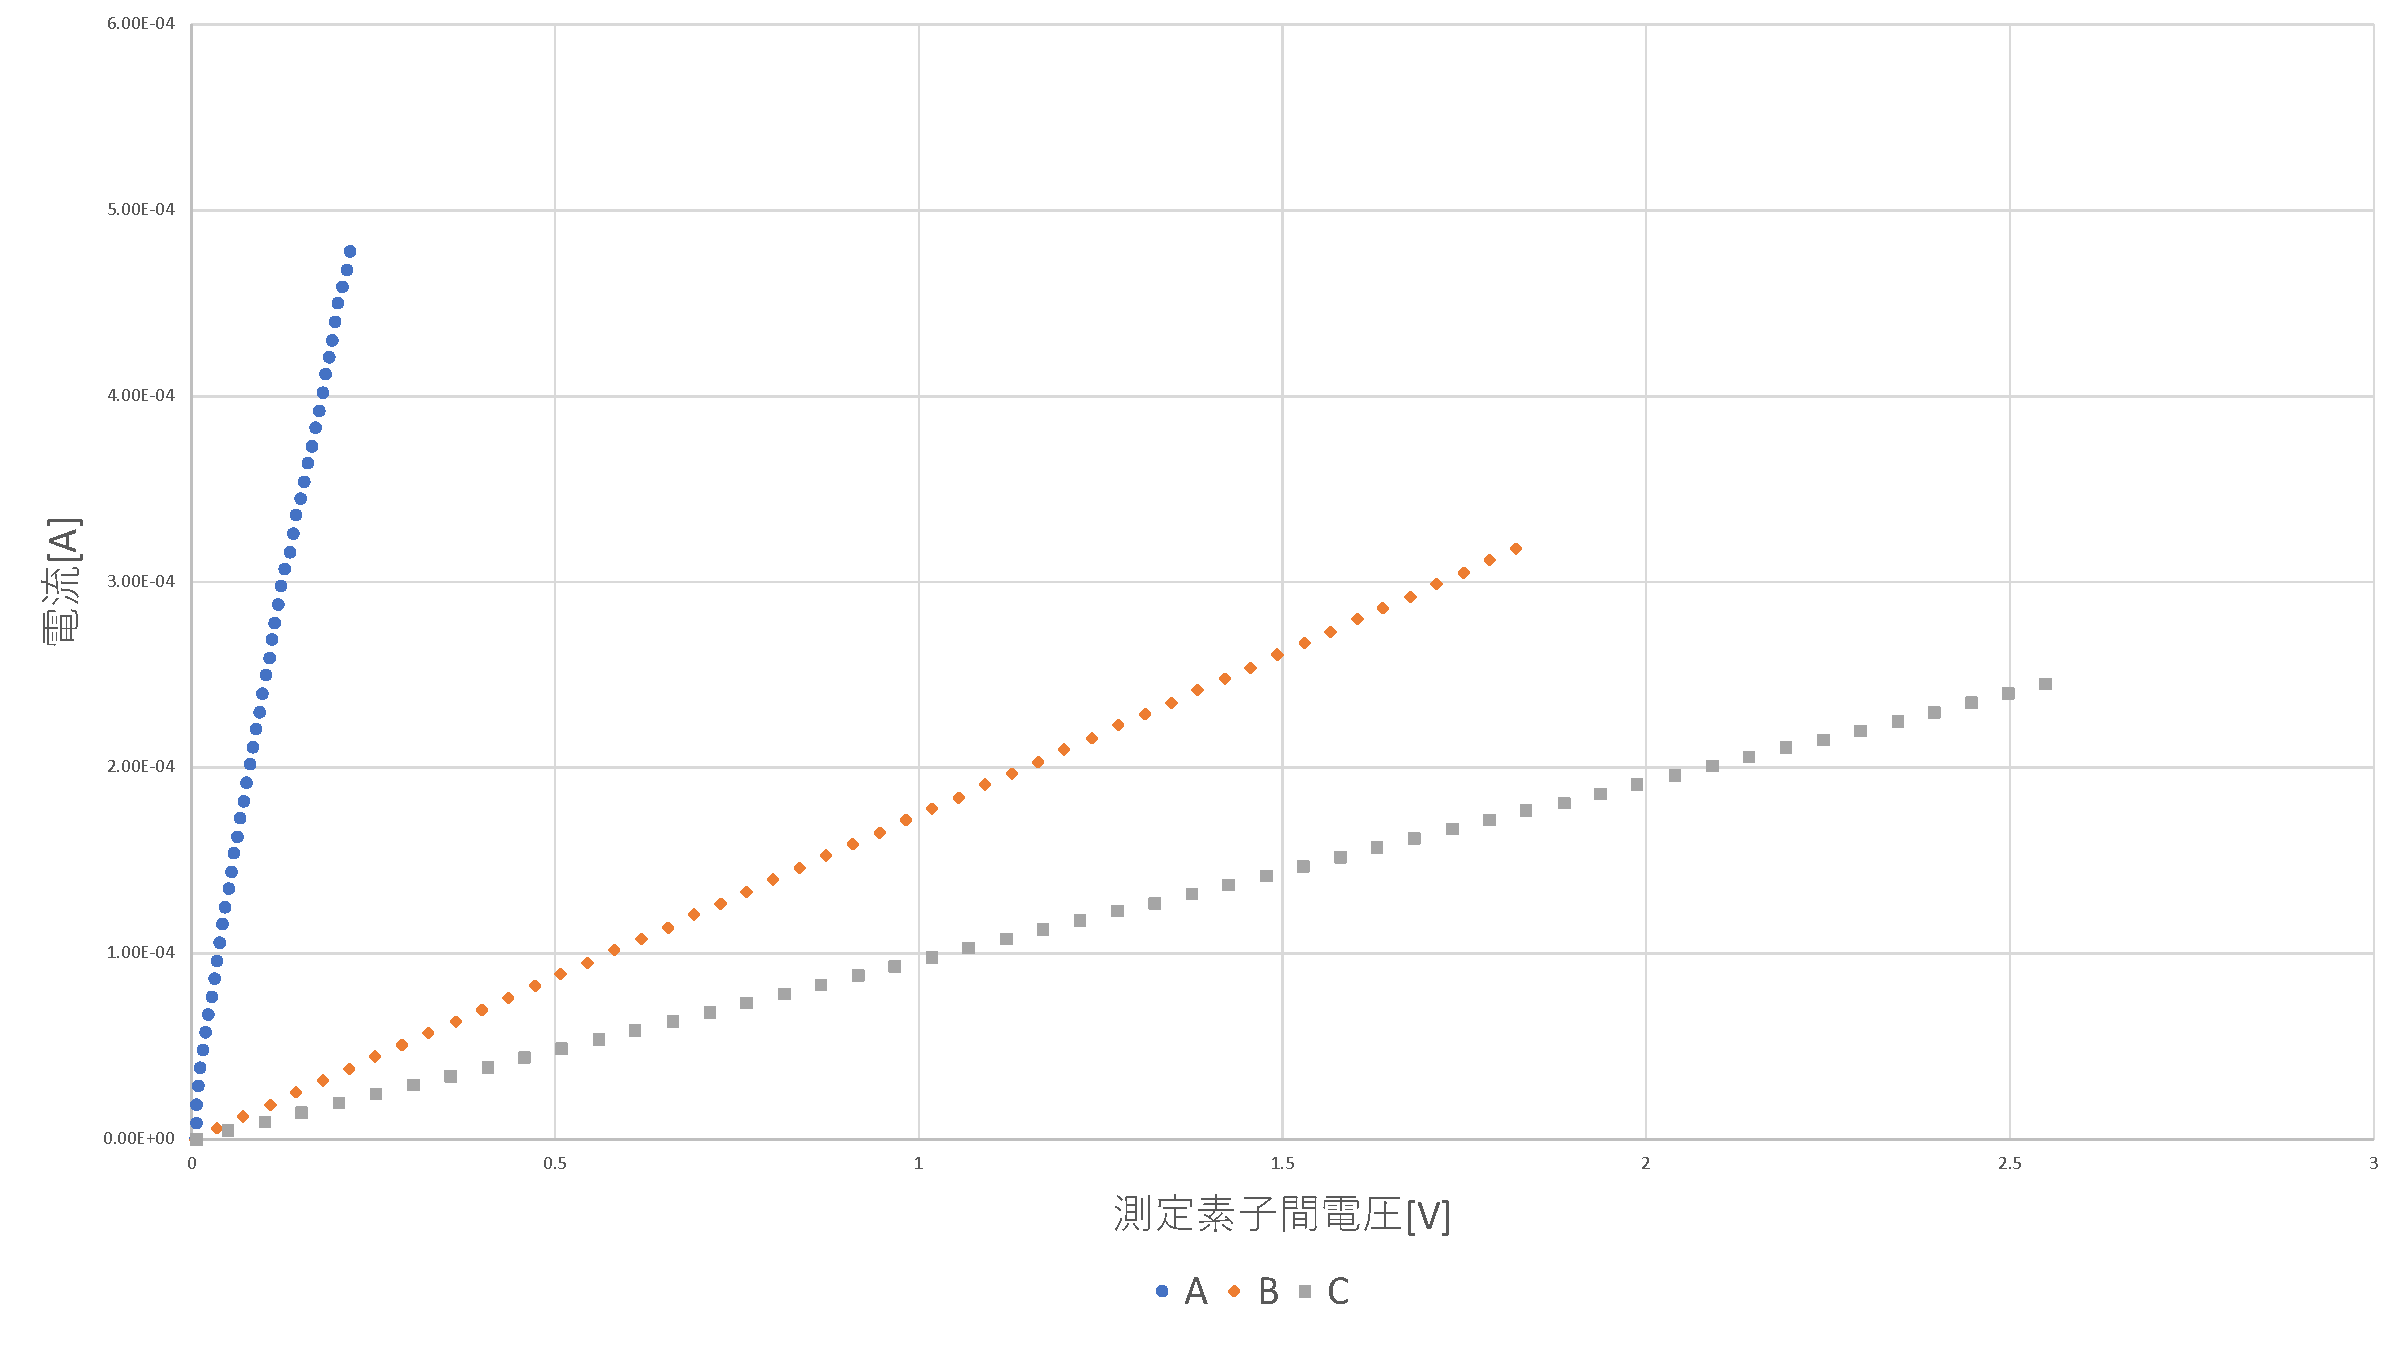
\includegraphics[scale=0.315]{./fig/3-2-2.pdf}}
	\caption{可変抵抗器(2-3端子間)の電圧電流特性}
	\label{fig:3-2-2}
  %\end{minipage}
  %\begin{minipage}[c]{0.5\hsize}
  \centering
  \centering
        \subfloat{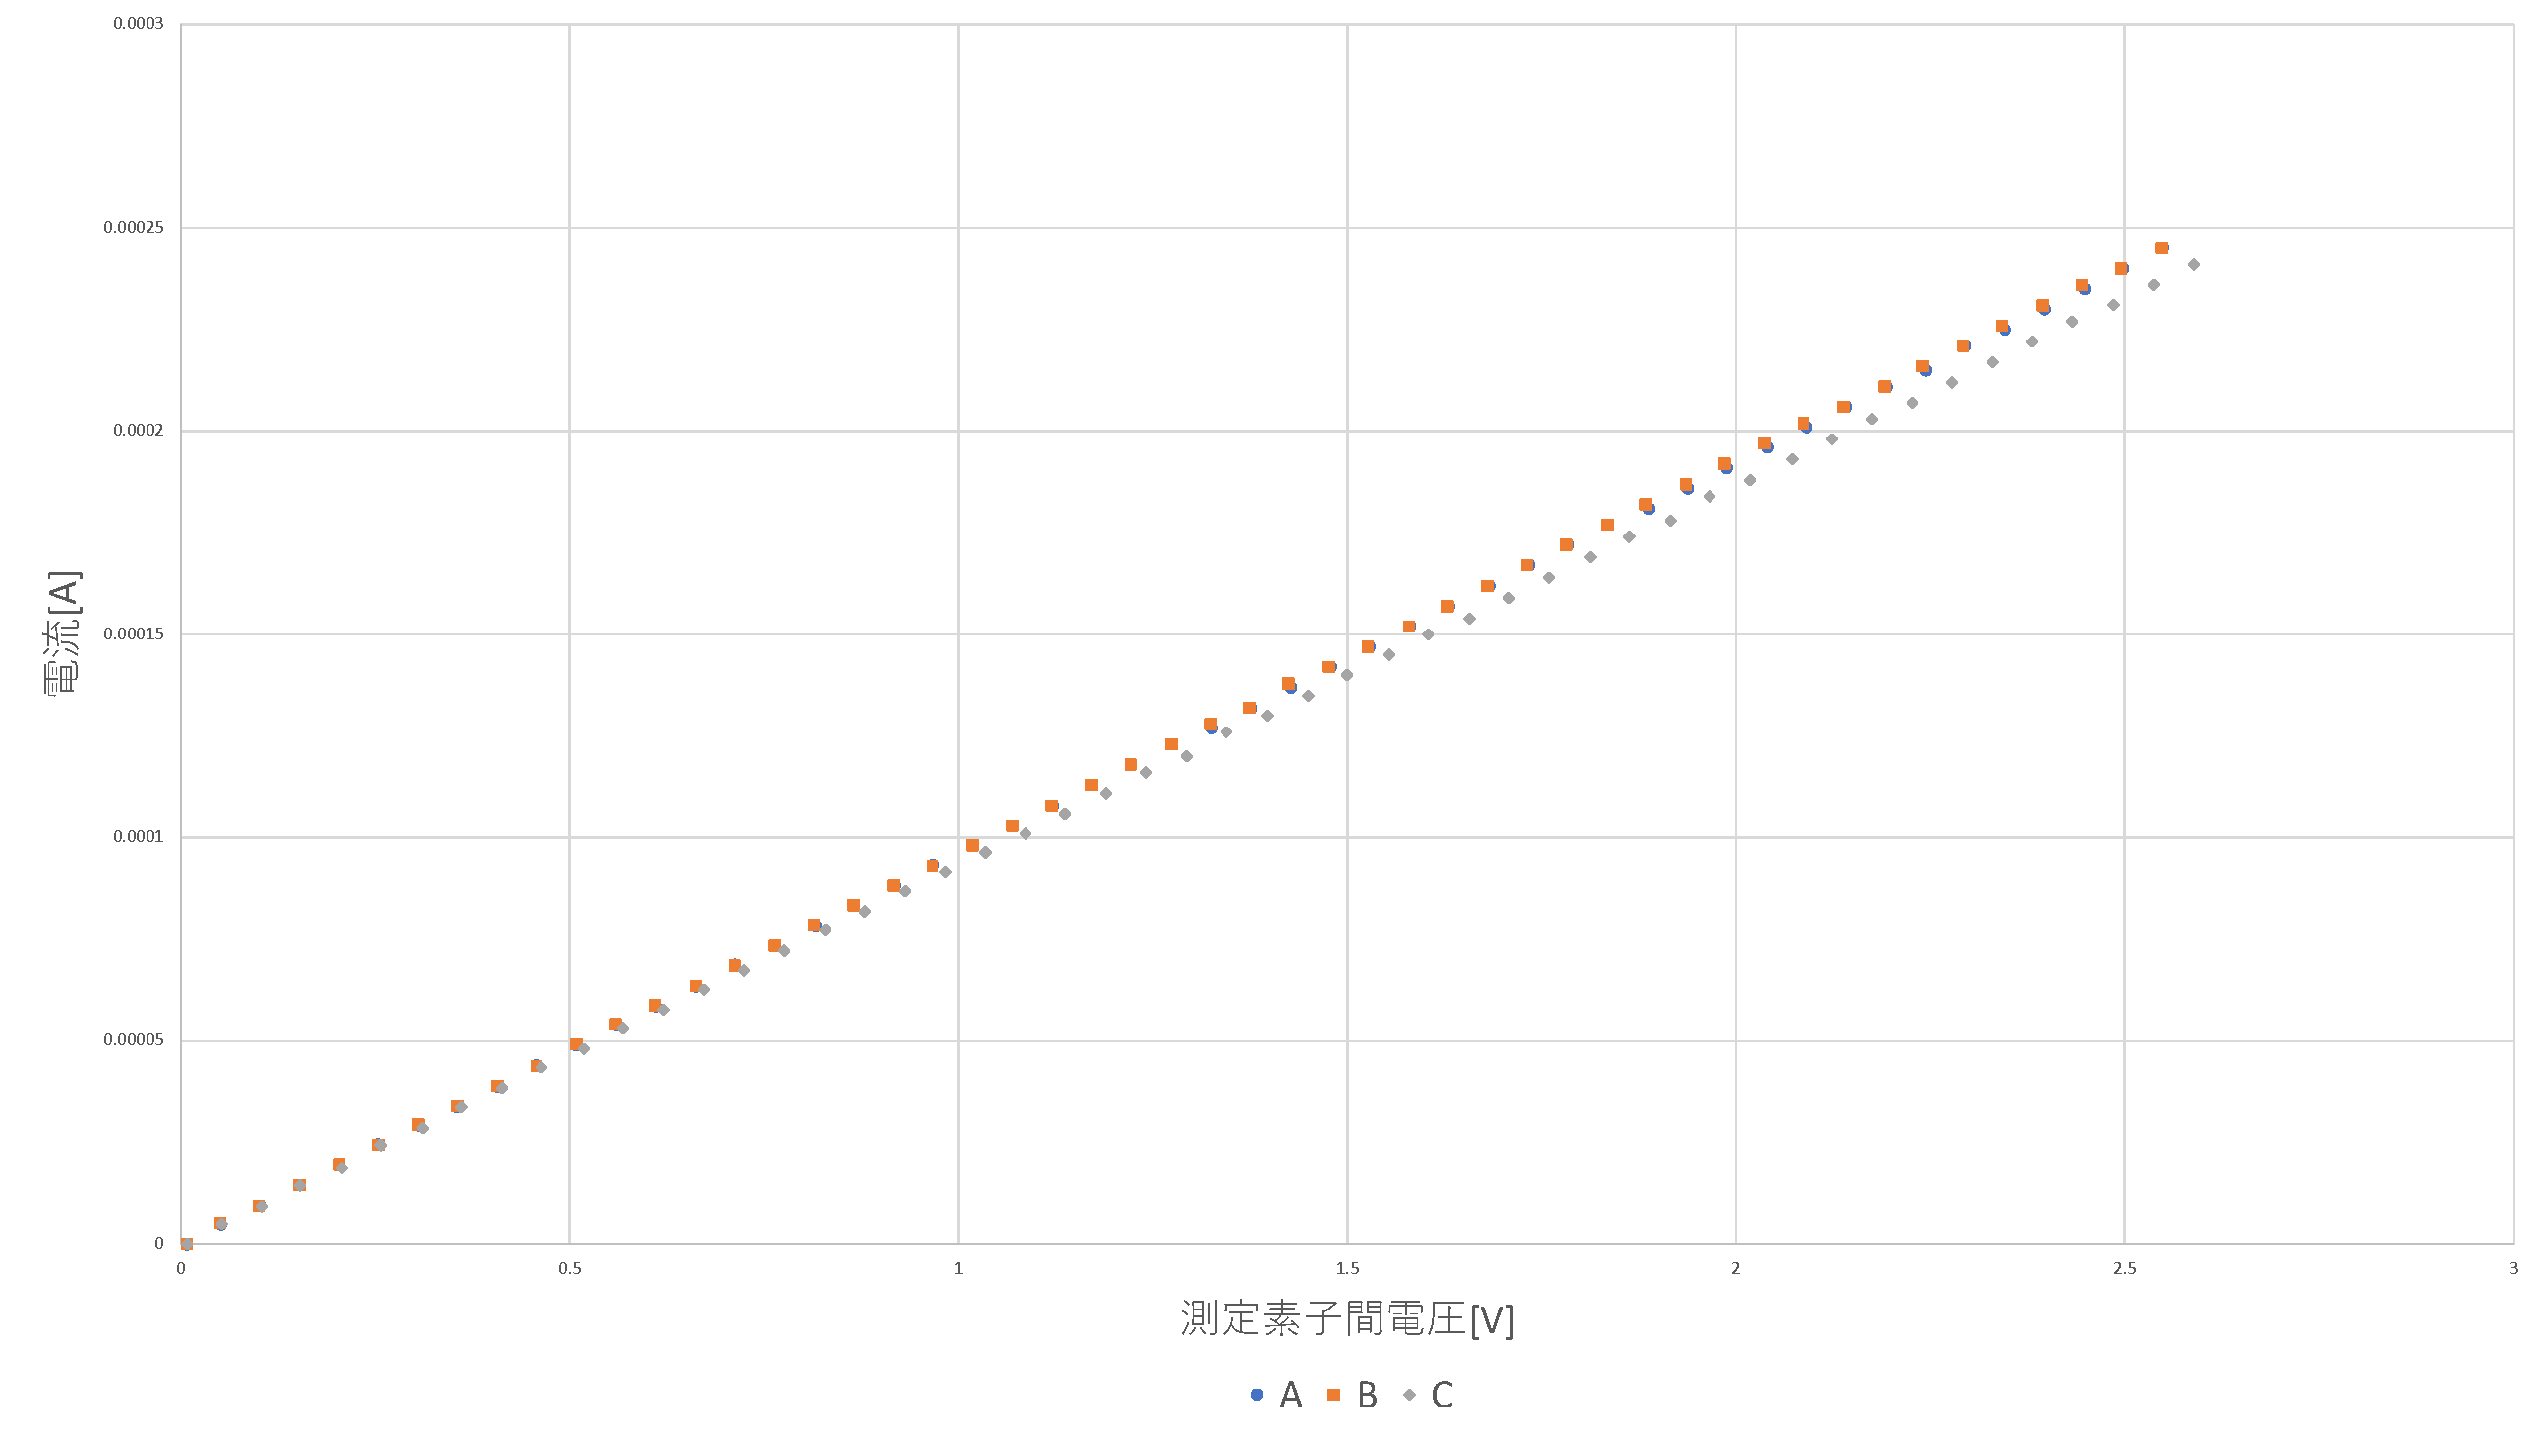
\includegraphics[scale=0.31]{./fig/3-2-3.pdf}}
	\caption{可変抵抗器(3-1端子間)の電圧電流特性}
	\label{fig:3-2-3}
 %\end{minipage}
\end{figure}